\begin{thm}{208}{\hosi 6}{東大OP 文系}
 座標平面において、原点Oを中心とする半径1の円C上に2点A$(1,0)$, B$(0,-1)$をとり、点PはCの$x>0, y>0$の部分を全て動く。直線PBと$x$軸との交点をQとし、$\triangle\mr{APQ}$の外心をRとする。Rの軌跡を求め、図示せよ。
\end{thm}

\begin{wrapfigure}[13]{r}[0pt]{100pt}
 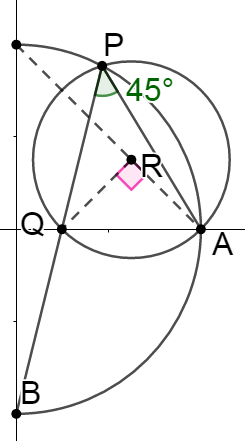
\includegraphics[width=\linewidth]{../problems/Q_208/A_208.png}
\end{wrapfigure}
$\angle\mr{AOB}=90^\circ$より、円周角の定理から$\angle\mr{BPA}=\angle\mr{QPA}=45^\circ$。$\triangle\mr{APQ}$の外接円上で、$\angle\mr{QPA}$は弧QAに対する円周角なので、$\angle\mr{QRA}=90^\circ$。点Rは外心なので、$\mr{RQ}=\mr{RA}$だから$\triangle\mr{QRA}$は直角二等辺三角形。

$\mr{P}(s, t)$とする ($s^2+t^2=1$, $s, t>0$)。直線PBは $y=\dfrac{t+1}{s}x-1$ より、 $\mr{Q}\left(\dfrac{s}{t+1}, 0\right)$ 。点Rの$x$座標はAQの中点の$x$座標に等しいので、 $\dfrac{1}{2}\left(1+\dfrac{s}{t+1}\right)$ であり、$y$座標は$\dfrac{1}{2}\mr{AQ}$に等しいので、 $\dfrac{1}{2}\left(1-\dfrac{s}{1+t}\right)$ である。 $m=\dfrac{s}{2(t+1)}$ として、 $\mr{R}\left(\dfrac{1}{2}+m, \dfrac{1}{2}-m\right)$ 。ここで、
\[ m=\frac{1}{2}\frac{\sqrt{1-t^2}}{t+1}=\frac{1}{2}\sqrt{\frac{1-t}{1+t}}=\frac{1}{2}\sqrt{\frac{2}{1+t}-1} \]
と、$0<t<1$から、$m$は$0<m<\dfrac{1}{2}$の範囲全体を動く。

$X=\dfrac{1}{2}+m$, $Y=\dfrac{1}{2}-m$として、$Y=-X+1$, $\dfrac{1}{2}<X<1$, $0<Y<\dfrac{1}{2}$なので、点Rの軌跡は、線分 $y=-x+1$~$\left(\dfrac{1}{2}<x<1\right)$。